
\subsection{Point cloud registration}
\label{sec:registration}


%We achieve the depth data from the 2 NIR cameras using depth estimation methods~\cite{Bleyer2011PatchMatch}.
After the global optimization, we get a set of camera parameters with minimal reprojection error.
However, there are still many problems in the 3D model obtained from directly merging the partial point clouds estimated from different views according to the estimated camera poses, mainly due to the low quality of depth estimation.
%
%If the depth and camera parameters are both accurate enough, the point clouds of different views should align very well.
%
While our global calibration step provides highly accurate camera poses, the point clouds from neighboring camera pods are close to each other in a coarse level.
The misalignment typically occurs at some parts of the human body, such as the head and arms, due to the depth estimation error in theses regions.
%
Therefore, we use the Iterative Closest Point (ICP) algorithm~\cite{Besl1992A} to slightly adjust the rigid transformation between two partial point clouds, and fuse the transformed point clouds to balance out the depth errors.
%

We choose the point cloud of one view as the reference, and align the point cloud of one of its neighboring views to it using the ICP algorithm. We combine the point clouds of the two views after that. Then we choose another neighboring view and do the registration sequentially. When all the point cloud of different views are registered, a high-quality 3D model can be achieved, as shown in Fig.~\ref{fig:3Dmodel}.
\begin{figure}[ht]
%
\begin{minipage}[b]{.48\linewidth}
  \centering
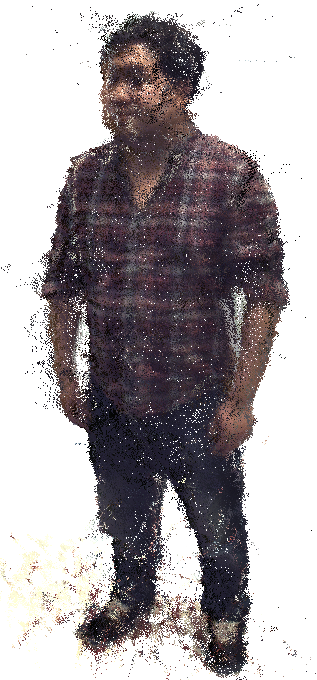
\includegraphics[width=3.cm]{image/model_front.png}
  \vspace{0cm}
  \centerline{(a)}\medskip
\end{minipage}
\hfill
\begin{minipage}[b]{0.48\linewidth}
  \centering
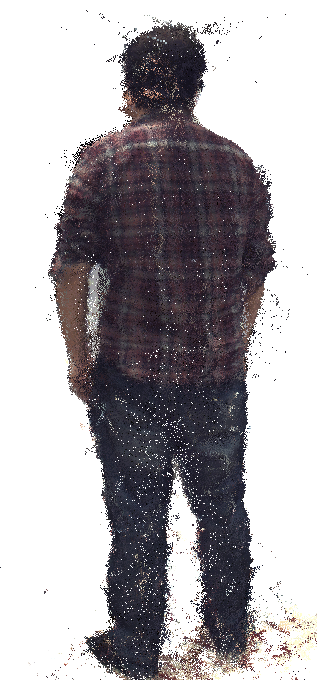
\includegraphics[width=3.cm]{image/model_back.png}
  \vspace{0cm}
  \centerline{(b)}\medskip
\end{minipage}
%
\caption{The 3D model after the registration. (a): The front of the model. (b): The back of the model. }
\label{fig:3Dmodel}
\end{figure}


\comments{
Most depth-estimation techniques based on NIR cameras are not robust enough, especially for light-absorbing materials like black hair.
Moreover, the depth estimation may be affected by many factors like the quality of the laser pointer, the interaction effect on the camera pods which are arranged towards each other caused by the laser and similarity.
%Although there have been many research on it, the error cannot be avoided completely.
As Fig.~\ref{fig:deptherror} shows, the estimated depth encounters large distortions on the boundary of the human body, and missing data in the head area.
Directly merge the point clouds estimated from 8 views according to the estimated camera parameters leads to a noisy and distorted point cloud, as Fig.~\ref{fig:} (a)(b) shows.\md{ToDo}


The point clouds reconstructed from different views are quite close to each other because of the global calibration, hence there is no need for the coarse registration.
We tried the state-of-the-art global registration algorithms~\cite{Evangelidis-ECCV-2014} to register all the point clouds from different views simultaneously without the corresponding points. However, the point clouds produced by our multi-camera system may have no overlapping fields, which leads to the wrong results. For example, the point cloud of the back of a human body may be aligned to the front overlappingly because of the symmetry of the shape of the body. To avoid these kinds of mistakes, we register the point clouds in multi views sequentially.
}

\comments{
In this registration step, we \emph{fuse} the partial point clouds reconstructed from each view using the
We choose the point cloud of one view as the reference, and align the point cloud of its neighboring views sequentially, using the Iterative Closest Point algorithm. \xj{Add the reference. If do not considering the time, why don't you use other state-of-the-art algorithms?}
The registration step is to minimize the distance between the corresponding points in different views mainly caused by the depth maps, which can be defined as:
\begin{equation}
E(\mathbf{R},\mathbf{T})=\sum_{N}(\mathbf{P}_{t}-\mathbf{R}\times\mathbf{P}_{s}-\mathbf{T})^{2},
\end{equation}
where $\mathbf{P}_{t}$ and $\mathbf{P}_{s}$ are a pair of corresponding points in the point clouds of the two views, N is the total number of the corresponding points, $\mathbf{R}$ and $\mathbf{T}$ represents the rigid transform, $\mathbf{R}$ is the rotation matrix and $\mathbf{T}$ is the translation matrix.

After the registration step, the point cloud which are not aligned very well because of the depth maps can be registered and a high-quality 3D model can be achieved.


Moreover, although the reprojection error after the global optimization mentioned in the last section is at sub-pixel level, which can prove the high accuracy of our calibration result, we still find the separation between the point cloud of different views when we map the depth to the entire model, effecting the quality of reconstruction. These deficiencies are mainly caused by the depth estimation.




To achieve a high-quality reconstruction, we fuse partial point clouds which are inaccurate and incomplete into a 3D model in a registration manner.
%
For each point reconstructed by the depth image, we consider an estimation.
\begin{equation}
\mathbf{\tilde{P}}_{ij}=f_{i}(\mathbf{P}_{j}),
\end{equation}
where $\mathbf{P}_{j}$ is the true 3D coordinates in the camera coordinate system. $f_{i}$ is a nonlinear function for view $i$, represent the depth influence. $\mathbf{\tilde{P}}_{ij}$ is the 3D coordinates we get from the depth data and intrinsic parameters in view $i$. With the extrinsic parameter, we can transform all the points into the world coordinate system. The estimation can be written as
\begin{equation}
\mathbf{\hat{P}}_{gj}=g(\mathbf{K_{ex}}_{i})f_{i}(\mathbf{P}_{j}),
\end{equation}
where $\mathbf{\hat{P}}_{gj}$ is the 3D coordinates in the world coordinate system we reconstruct from the depth and camera parameters. ICP can be replaced as a rigid transform to all views
\begin{equation}
\mathbf{\tilde{\hat{P}}}_{gj}=M_{i}g(\mathbf{K_{ex}}_{i})f_{i}(\mathbf{P}_{j})=g(\mathbf{K_{ex}}_{i})M_{i}f_{i}(\mathbf{P}_{j}),
\end{equation}
where $\mathbf{\tilde{\hat{P}}}_{gj}$ is the coordinates of the point after the alignment. The transform $M_{i}$ can refine the error caused by $f_{i}$, and improve the quality of the result of 3D reconstruction.
}%

% view 2 to it, combine the result of the two views, then align the point cloud of view 3 to the combined result and so on.
%Each ICP process produce a transformation matrix, then we can map the inaccurate depth to a high-quality 3D model using the rigid transformation.


